%\setverb\setnash
%\hyphenpenalty=10000
%\sloppypar
%\begin{document}
\chapter{METODOLOGI PENELITIAN}\label{cha:metodologi}
%\pagenumbering{arabic}
%\AddToShipoutPicture{\BackgroundPic}
%\DeclareUnicodeCharacter{FFFD}{?????}
\section{Alat yang Digunakan}\label{sec:alat}
\subsection{Perangkat Keras}\label{sec:perangkatk}
\hspace{0.6cm}Perangkat keras yang digunakan adalah sebuah laptop dengan spesifikasi sebagai
berikut:

\begin{table}
\centering
\caption{Spesifikasi Perangkat Keras.}
\begin{center}
\begin{tabular}{|c|c|c|}
\hline
No & Komponen & Spesifikasi \\
\hline
1 & Processor & Intel(R) Core(TM) i5-4300M CPU @ 2.60GHz 2.59 \\
\hline
2 & Memory & 12GB \\
\hline
3 & Display & Intel(R) HD Graphics 4600 \\
\hline
4 & Renderer & - \\
\hline
5 & OS & Windows 10 \\
\hline
\end{tabular}
\end{center}
\end{table}

\subsection{Perangkat Lunak}\label{sec:perangkatl}
\hspace{0.6cm}Perangkat lunak yang digunakan :

\begin{table}
\centering
\caption{Spesifikasi Perangkat Lunak.}
\begin{center}
\begin{tabular}{|c|c|c|}
\hline
No & Komponen & Software \\
\hline
1 & Text Editor & Sublime \\
\hline
2 & Browser & Google Chrome \\
\hline
3 & \emph{Library} & victor js \emph{library} \\
\hline
\end{tabular}
\end{center}
\end{table}

\hspace{0.6cm}Perangkat keras pada Tabel 3.1 adalah milik pribadi penulis. Meninjau simulasi
akan menggambar banyak partikel yang dihitung terus menerus maka graphic card dan RAM yang digunakan sebaiknya tidak jauh berbeda dengan yang dimiliki
penulis. Adapun perangkat lunak pada Tabel 3.2 yang digunakan dapat ditemukan
secara gratis di internet



\section{Penerapan Gaya}

\subsection{Penerapan 3 gaya}
\hspace{0.6cm}Pola \emph{flocking} dimana partikel diproyeksikan bergerak membentuk formasi berkelompok sesuai dengan grupnya.Untuk hal tersebut diterapkan partikel disimulasikan dalam kasus dimana partikel dimunculkan pada tempat yang acak. setelahnya partikel akan bergerak dipengaruhi 3 gaya yaitu \emph{alignment}, \emph{cohesion}, dan \emph{separation}. Sampai pola gerak berkelompok terbentuk

\subsection{Penerapan 3 gaya ditambah gaya \emph{circular}}

\begin{equation}
\vec{F}_i = \vec{F^a}_i + \vec{F^k}_i + \vec{F^s}_i + \vec{F^c}_i
\end{equation}

\hspace{0.6cm}Pada kasus dengan tambahan gaya 
\emph{circular}, partikel akan diterapkan gaya pusat \emph{circular} sebagai prioritas agar partikel bergerak didalam area tawaf. dan ketika berada diarea tawaf partikel bergerak secara \emph{circular} berlawanan arah jarum jam. dalam area tawaf ada gaya yang sama untuk mencegah agar partikel tetap berada di area tawaf.
untuk prioritas gaya maka ada massa \emph{factor} (m) sebagai besar \emph{factor} prioritasnya.

\begin{equation}
\vec{F}_i = m^a\vec{F^a}_i + m^k\vec{F^k}_i + m^s\vec{F^s}_i + m^c\vec{F^c}_i
\end{equation}

\subsubsection{interaksi diluar zona tawaf}
\hspace{0.6cm} Maksud dari interaksi diluar tawaf. adalah partikel hanya bergerak menuju ke zona tawaf. Dengan gaya partikel lain yang minim. Hal ini menggiring partikel menuju pergerakan di area tawaf.

\subsubsection{interaksi didalam zona tawaf}
\hspace{0.6cm} Pada kasus ini partikel berinteraksi dengan grup partikel lain, juga berinteraksi dengan partikel yang berbeda grup juga. Partikel dengan grup sama diwakilkan dengan warna yang sama mempunyai gaya separasi yang lebih kecil dibandingkan dengan partikel yang berbeda grupnya. 

Adapun gaya circular dalam simulasi digunakan untuk partikel melakukan putaran tawaf. \emph{Flocking}juga dapat distabilkan jika kelompok partikel berkumpul dengan sejenisnya, Membentuk grup sambil melakukan tawaf. Hal ini mencerminkan partikel menjaga eksistensi grupnya, sambil melakukan tawaf.

\section{Simulasi Komputer}
\hspace{0.6cm}Simulasi dan program dibagun dalam bahasa \emph{JavaScript} sebagai dasar \emph{source code}. secara visual menampikan animasi dan grafik yang menghasilkan outputnya.Bentuk matematis program dimuat dalam \emph{library} Victorjs. Dimana fungsi kalkulasi vektor terdapat dalamnya, sehingga dapat dipanggil dengan mudah.

\begin{table}
\centering
\caption{Sekilas tentang pengunaan \emph{library} VictorJS .}
\begin{center}
\begin{tabular}{|c|c|}
\hline
Penulisan koordinat  & Penulisan koordinat\\
gaya menggunakan victorjs &  gaya tanpa victor js menggunakan array javascript\\
\hline
var Vector = new Victor(diff.x,diff.y); & var Vector = [diff.y,diff.y] \\
\hline
\hline
sum.add(Vector) & Vector = [diff.y,diff.y] + [sum.y,sum.y]  \\
\hline
\end{tabular}
\end{center}
\end{table}

\hspace{0.6cm}Tabel diatas menggambarkan penulisan Koordinat menggunakan \emph{library} Victor.js\citep{noauthororeditor2014victorjs}. Gaya berbentuk array dalam program biasa dapat dikonversi kedalam \emph{library} menggunakan victor.js, di dalam victor.js juga terdapat perintah untuk menjumlahkan gaya dengan singkat seperti terdapat pada no 2. Terdapat banyak lagi selain penjumlahan vector, pengurangan, akar kuadrat dan lain-lain.  



\begin{figure}
\centering
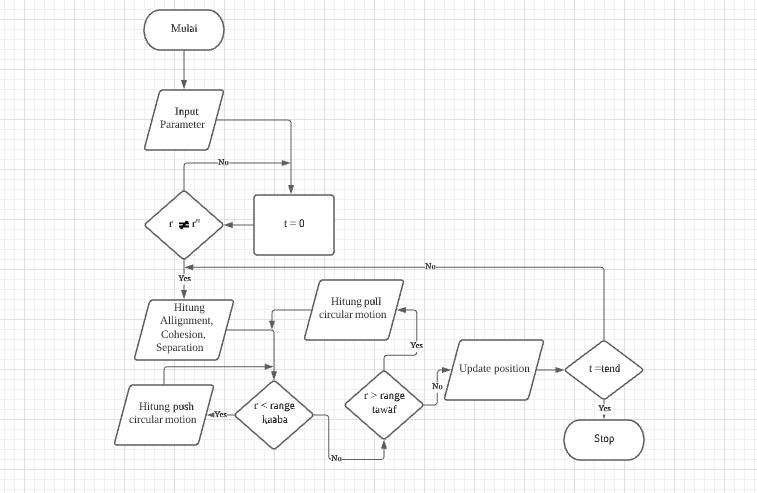
\includegraphics[scale=0.75]{gambar/diagram} %gambarnya harus algoritma
\caption{Algoritma Pemograman.}
\end{figure}

\section{Parameter Gaya}
% Parameter gaya dijabarkan pada bab 2 diantaranya
\subsection{Parameter dalam pergerakan gaya}
\hspace{0.6cm}Dalam penerapannya, hasil simulasi kaaba diletakan di pusat dengan titik (sekian) dimana parameter penting lainnya adalah koordinat partikel yang dimunculkan secara acak dalam ruang interaksi zona tawaf maupun zona diluar tawaf. Partikel juga memiliki sebuah id untuk mengkatagorikan partikel dalam sebuah kelompok. Parameter selajutnya adalah gaya antar partikel yang diatur agar partikel membuat sebuah grup, dalam hal ini, gaya separasi yang (koefisien \emph{boid} < koefisien partikel lain) akan membuat partikel memilih jarak yang yang berbeda sesuai dengan grup partikelnya. parameter lain yang berpengaruh adalah gaya tarik kedalam zona tawaf agar partikel membuat gerakan tawaf. Jumlah partikel N ditentukan untuk menguji kestabilan simulasi dalam hal ini dibatasi dengan jumlah orde 3 digit untuk menghindari adanya laging dalam proses simulasinya.

Dalam \emph{interface}, gaya separasi dibentuk dari salah satu variabel yaitu jarak separasi($z_s$) didalamnya dalam  terdapat koefisien introversi dan koefisien rasis dimana koefisien ini membentuk radius maksimum untuk melakukan gaya separasi dimana \emph{desiredSeparation} = radius \emph{boid} + radius \emph{boid} lain + ( 25 * koefisien \emph{introversion} ) + ( 50 * \emph{racismMultiplier} koefisien ). Pada koefisien \emph{racism} diterapkan logika bahwa jika partikel memiliki warna sama maka koefisien \emph{racism} akan menjadi nol, dan jika tidak maka akan mempunyai nilai. Nilai ini yang mengaktifkan gaya separasi.

Parameter lain yang mempengaruhi gaya adalah jarak pensejajaran $z_a$, dimana ada aturan jarak yang dibutuhkan untuk gaya mempengaruhi \emph{boid} agar melakukan pensejajaran dengan \emph{boid} lain parameter jarak ini adalah 25.

Parameter lain yang mempengaruhi gaya adalah jarak kohesi$z_k$, dimana ada aturan jarak yang dibutuhkan untuk gaya mempengaruhi \emph{boid} agar melakukan kompresi dengan \emph{boid} lain parameter jarak ini adalah 25.
\subsection{Parameter variasi partikel yang ditambahkan dalam simulasi}
Pada simulasi ditambahkan partikel dengan kecepatan yang berbeda. Terdapat 3 variasi kecepatan yang digunakan diantaranyaa \emph{quickness} = 1 , \emph{agroQuickness} = 1.25 dan \emph{blackQuickness} = 0.5. Pada partikel yang merah ditentukan parameter kecepatan yang 1.25 koefisien dari kecepatan normal. Pada partikel hitam ditentukan koefisien nya yaitu 0.45 dari kecepatan normal.
% \subsection{Perhitungan koefisien introversion dan rasisme}
% \hspace{0.6cm}untuk mendapatkan nilai koefisien yang diperlukan gaya diperlukan nilai distribusi normal untuk menjaga sebuah koefisien setiap simulasi dijalankan berbeda tetapi tidak membuat simulasi tidak stabil.

% dengan persamaan 2.6 kalkulasi koefisien dari introversion and rasisme dapat dikalkulasikan, nilai dari variabel mean adalah 50 dan standard deviasinya adalah 9.


%tes \citep{wannamaker04}

%\end{document}